\documentclass[12pt]{article}

% Packages
\usepackage[utf8]{inputenc}
\usepackage[T1]{fontenc}
\usepackage{lipsum} % For generating dummy text
\usepackage[margin=2cm]{geometry} % Adjust the margin size here
\usepackage{amsmath}
\usepackage{graphicx}
\usepackage{mdframed}
\usepackage{hyperref}
\usepackage{amssymb}



% Title and author
\title{NLP CS5803 IITH Notes}
\author{Deepak}

\begin{document}

\maketitle
\tableofcontents

\newpage

\section{Introduction}
The starting question is how to make computers understand human
language. We need to find smart ways of representing the language.

\section{Input Representation}
    Consider text modality, where the input is a document, it
    consists of words(also called tokens). The document is represented
    by the set of words/tokens it contains.

    Lets see some methods for text representation
    

    \subsection{TF-IDF scheme}

        \subsubsection{Formulation}
            The TF-IDF (Term Frequency-Inverse Document Frequency) scheme is a
            popular technique used to represent the importance of words in a 
            document corpus. \\
            It combines two factors: term frequency (TF) and inverse document frequency (IDF). \\
            \textbf{TF} measures the frequency of a term in a document. 
            It is calculated by counting the number of occurrences of a term 
            in a document as a raw or by taking a log of it.

            \[
            \text{tf}(t, d) = \begin{cases}
                            0 & \text{if } c(t, d) = 0 \\
                            1 + \log(c(t, d)) & \text{if } c(t, d) \neq 0
                        \end{cases}
            \]

            where $c(t, d)$ is the count of term $t$ in document $d$.
            \\
            \textbf{IDF} de-emphasizes the frequent words across the corpus
            (all documents combined is usually called corpus) and emphasizes
            the on words differentiating the documents.

            \[
            \text{idf}(t) = \log_{10} \left( \frac{N}{\text{df}_{t}}\right)
            \]
            
            where $N$ is the total number of documents in the corpus and $\text{df}_{t}$ is the number of documents containing the term $t$.
            \\
            The TF-IDF score for a term in a document is obtained by multiplying its TF value with its IDF value. Mathematically, it can be represented as:

            \[
            \text{tf-idf}(t, d) = \text{tf}(t, d) \times \text{idf}(t)
            \]
            Now we get a table with TF-IDF values.
            
            This way, each document is represented by a vector from the column
            of the table and each word is presented by a vector from
            the row of the table.

            \subsubsection{Limitation}
            \begin{itemize}
                \item Words are considered at their lexical appearance
                \item Synonymy is not considered
                \item Polysemy(word with multiple meanings) is not considered
                \item long sparse vectors
                \item context is not considered
            \end{itemize}

    \subsection{SVD - text representation}
        \subsubsection{Formulation}
            Consider the term-document matrix and apply SVD to it
            to do dimensionality reduction, so that we can get dense
            representations.
            \\
            Let A be the term-document matrix(matrix with freq. of words in docs), 
            where each row represents a term and each column represents a document, 
            by SVD we have

            \[
                A = U \Sigma V^{T}
            \]
            U, V are orthonormal matrices and $\Sigma$ is a diagonal matrix of 
            singular values of A in decreasing order.
            \\
            By keep only the first k singular values, we have

            \[
                A_k = U_k \Sigma_k V_k^{T}
            \]

            The k here is much smaller than the original dimension of A.
            Terms can be represented by the rows of $U_k$ and documents can be
            represented by the columns of $V_k$.
            
    \subsection{LDA - text representation(incomplete)}
        \subsubsection{Formulation}
            LDA (Latent Dirichlet Allocation) is a text representation based
            on \textbf{topics}. It assumes that each document is a mixture of 
            topics which are latent or unknown. Words in a document depend on
            topics of the document. LDA is a mechanism to identify the topics
            and connect words with topics
            \\
            The generative process is as follows:
            \begin{itemize}
                \item For each document, draw a distribution over topics
                \item For each word in the document, draw a topic from the
                distribution over topics and then draw a word from the
                distribution over words for that topic.
            \end{itemize}
            The parameters of the model are the topic distributions for each
            document, the word distributions for each topic, and the topic
            distribution over the entire corpus.
            \\
            The model is trained by maximizing the likelihood of the observed
            documents. The topic distributions for each document and the word
            distributions for each topic are learned from the data.
            \\
            The learned topic distributions for each document can be used to
            represent the documents and the learned word distributions for each
            topic can be used to represent the topics.
            
        \subsubsection{Mathematical Formulation}

            The mathematical formulation of LDA is as follows:
            
            For each document $d$ in the corpus $D$:
            
            1. Choose $N \sim Poisson(\xi)$.
            
            2. Choose $\theta \sim Dir(\alpha)$.
            
            3. For each of the $N$ words $w$:
            
                a. Choose a topic $z \sim Multinomial(\theta)$.
            
                b. Choose a word $w$ from $p(w|z,\beta)$, a multinomial probability conditioned on the topic $z$.
            
            Here, $\xi$ is the parameter of the Poisson distribution used to choose the number of words in a document, $\alpha$ is the parameter of the Dirichlet distribution used to generate the per-document topic distributions, and $\beta$ is the parameter of the multinomial distribution used to generate the per-topic word distribution.
        

    \subsection{Word2Vec}
        \textbf{Context of words}: Context of a word is the set of words that surround it.
        For example, in the sentence "I love to eat pizza", the context of the word "love" is \{"I", "to", "eat"\}.
        \\
        Note: Word2Vec models rely on "distributional symmetry" hypothesis, i.e. similar words have similar contexts.
        \\
        Word2Vec is a popular technique used to represent words in a continuous vector space. \\
        It is based on the idea that words that appear in similar contexts are semantically similar.
        Word2Vec has two models: SkipGram and Continuous Bag of Words (CBOW).
        \begin{figure}[h]
            \centering
            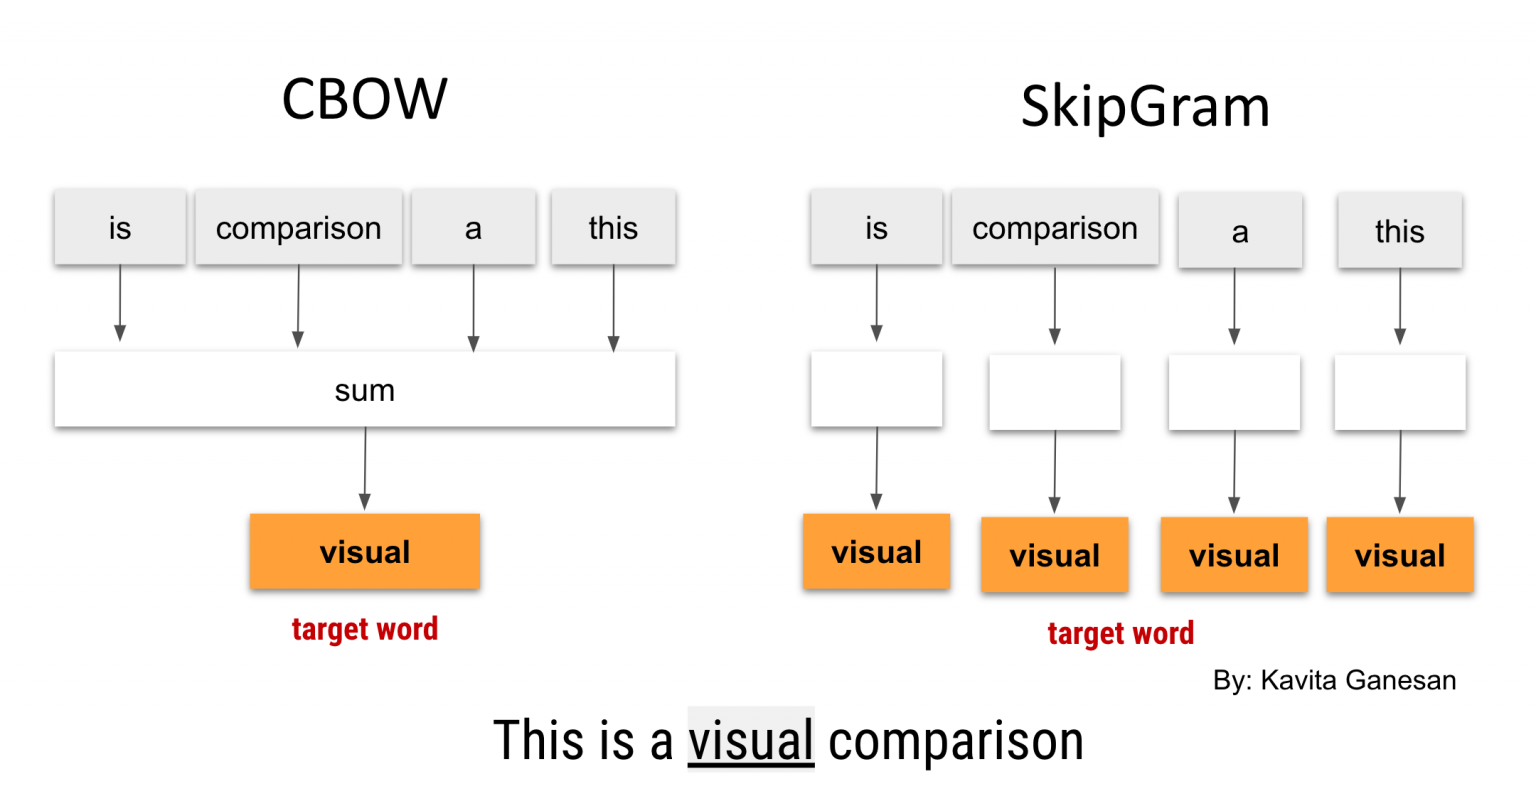
\includegraphics[width=0.5\textwidth]{/workspaces/DartBase/notes/nlp/images/cbow_vs_sg.png}
        \end{figure}
        \subsubsection{Continuous Bag of Words (CBOW)}
            This model predicts the middle word based on the context words.
            
            We create two matrices, $V \in \textbf{R}^{n \times |V|}$ and $U \in \textbf{R}^{|V| \times n}$. Where $n$ is an arbitrary size which defines the size of our embedding space.
            \begin{mdframed}
            $w_i$: Word $i$ from vocabulary $V$ \\
            $V \in \textbf{R}^{n \times |V|}$: Input word matrix \\
            $v_i$: $i_{th}$ column of $V$, the input vector representation of word $w_i$\\
            $U \in \textbf{R}^{n \times |V|}$: Output word matrix\\
            $u_i$: $i_{th}$ row of $U$, the output vector representation of word $w_i$
            \end{mdframed}
            Note that we do in fact learn two vectors for every word $w_i$ (i.e. input word vector $v_i$ and output word vector $u_i$).
            \begin{figure}[h]
                \centering
                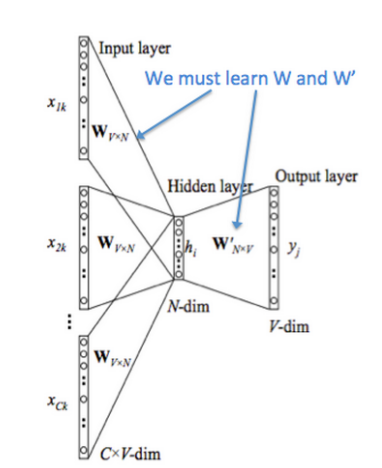
\includegraphics[width=0.5\textwidth]{/workspaces/DartBase/notes/nlp/images/cbow_net.png}
            \end{figure}
            also, the below steps are done using a single hidden layer neural network.\\
            We breakdown the way this model works in these steps:
            \begin{enumerate}
                \item We generate the one hot word vectors $(x_{c-m}, \ldots, x_{c-1}, x_{c+1}, \ldots, x_{c+m})$ for the input context of size $m$.
                \item We get our embedded word vectors for the context  \\
                $(v_{c-m} = Vx_{c-m}, v_{c-m+1} = Vx_{c-m+1}, \ldots, v_{c+m} = Vx_{c+m})$.
                \item Average these vectors to get $\hat{v} = \frac{v_{c-m} + v_{c-m+1} + \ldots + v_{c+m}}{2m}$.
                \item Generate a score vector $z = U\hat{v}$.
                \item Turn the scores into probabilities $\hat{y} = \text{softmax}(z)$.
                \item We desire our probabilities generated, $\hat{y}$, to match the true probabilities, $y$, which also happens to be the one hot vector of the actual word.
            \end{enumerate}
            
            Since, we have a neural network we need objective function.
            we use a popular choice of distance/loss
            measure, cross entropy $H(\hat{y}, y)$.

            \begin{align*}
                H(\hat{y}, y) &= -\sum_{i=1}^{|V|} y_i \log(\hat{y}_i) \\
                &= -\log(\hat{y}_j)\\
                &= - \log \frac{\exp(z_c)}{\sum_{j=1}^{|V|} \exp(z_j)} \\
                &= - \log \frac{\exp(u_c^T \hat{v})}{\sum_{j=1}^{|V|} \exp(u_j^T \hat{v})} \\
                &= - \log P(u_c|\hat{v}) \\
                &= - \log P(w_c|w_{c-m}, \ldots, w_{c-1}, w_{c+1}, \ldots, w_{c+m})
            \end{align*}
            
            Hence, it perfectly makes sense to choose the cross entropy as our loss function.
        
        \subsubsection{SkipGram}
            Predicting surrounding context words given the middle word.\\
            \begin{figure}[h]
                \centering
                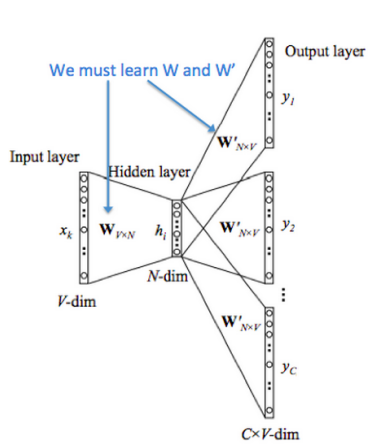
\includegraphics[width=0.5\textwidth]{/workspaces/DartBase/notes/nlp/images/sg_net.png}
            \end{figure}
            
            The setup is largely the same but we essentially swap our $x$ and $y$ i.e. $x$ in the CBOW are now \\ $y$ and vice-versa. 
            The input one hot vector (center word) we will represent with an $x$ (since there is only one). 
            And the output vectors as $y^{(j)}$. We define $V$ and $U$ the same as in CBOW.


            We breakdown the way this model works in these 6 steps:
            \begin{enumerate}
                \item We generate the one hot input vector $x$.
                \item We get our embedded word vectors for the input vector $v_c = Vx$.
                \item Generate the logits of size V using $u = Uv_c$.
                \item Turn the logits into probabilities, $\hat{y} = \text{softmax}(u)$.
                \item We desire to minimize the negative log likelihood of probabilities.
            \end{enumerate}
            
            As in CBOW, we need to generate an objective function for us to
            evaluate the model. 
            \begin{align*}
                J &= - \log P(w_{c-m}, \ldots, w_{c-1}, w_{c+1}, \ldots, w_{c+m}|w_c) \\
                &= - \log \prod_{j=0, j \neq m}^{2m} P(w_{c-m+j}|w_c) \\
                &= - \log \prod_{j=0, j \neq m}^{2m} P(u_{c-m+j}|v_c) \\
                &= - \log \prod_{j=0, j \neq m}^{2m} \frac{\exp(u_{c-m+j}^T v_c)}{\sum_{k=1}^{|V|} \exp(u_k^T v_c)} \\
                &= - \sum_{j=0, j \neq m}^{2m} u_{c-m+j}^T v_c + 2m \log \sum_{k=1}^{|V|} \exp(u_k^T v_c)
            \end{align*}

            Similar to CBOW this can also be written as error between $y^i$ and $\hat{y^i}$ .
        \subsubsection{Negative Sampling}
        Note that the
        summation over |V| is computationally huge! Any update we do or
        evaluation of the objective function would take O(|V|) time which
        if we recall is in the millions. This is where negative sampling comes
        to the rescue. The idea is to sample a small number of negative
        examples (words that are not in the context of the center word).

        While negative sampling is based on the Skip-Gram
        model, it is in fact optimizing a different objective.

        Consider a pair $(w, c)$ of word and context word.
        Let's denote by $P(D = 1|w, c)$ the probability that $(w, c)$ came from the corpus data. Correspondingly, $P(D = 0|w, c)$ will be the
        probability that $(w, c)$ did not come from the corpus data. First, let's model $P(D = 1|w, c)$ with the sigmoid function:
        \[P(D = 1|w, c, \theta) = \frac{1}{1 + e^{-v_c^T v_w}}\]
         
        Now, we build a new objective function that tries to maximize the probability of a word and context being in the corpus data if it indeed is, and maximize the probability of a word and context not being in the corpus data if it indeed is not. We take a simple maximum likelihood approach of these two probabilities. (Here we take $\theta$ to be the parameters of the model, and in our case it is $V$ and $U$.)

        \begin{align*}
            \theta &= \arg\max_{\theta} \prod_{(w,c) \in D} P(D = 1|w, c, \theta) \prod_{(w,c) \in \tilde{D}} P(D = 0|w, c, \theta) \\
            &= \arg\max_{\theta} \prod_{(w,c) \in D} P(D = 1|w, c, \theta) \prod_{(w,c) \in \tilde{D}} (1 - P(D = 1|w, c, \theta)) \\
            &= \arg\max_{\theta} \sum_{(w,c) \in D} \log P(D = 1|w, c, \theta) + \sum_{(w,c) \in \tilde{D}} \log(1 - P(D = 1|w, c, \theta)) \\
            &= \arg\max_{\theta} \sum_{(w,c) \in D} \log \frac{1}{1 + \exp(-u_w^T v_c)} + \sum_{(w,c) \in \tilde{D}} \log\left(1 - \frac{1}{1 + \exp(-u_w^T v_c)}\right) \\
            &= \arg\max_{\theta} \sum_{(w,c) \in D} \log \frac{1}{1 + \exp(-u_w^T v_c)} + \sum_{(w,c) \in \tilde{D}} \log\left(\frac{1}{1 + \exp(u_w^T v_c)}\right)
        \end{align*}
        This changes as follows by considering k negative samples for each postive.
        \[
            \log \sigma(u_{c-m+j}^T v_c) + \sum_{k=1}^{K} \log \sigma(-\tilde{u}_k^T v_c)
        \]
        In the above formulation, $\{\tilde{u}_k | k = 1, \ldots, K\}$ are sampled from $P_n(w)$.
        the n value of 0.75 seems work well in practice, since it increase the high probability words 
        less, while low probability words more.

    \subsection{GloVe}
        \subsubsection{Formulation}
            Emphasizes on co-occurrence with context/ Probe word 
            \begin{mdframed}
                Co-occurrence Matrix:
                \begin{itemize}
                    \item $X$: word-word co-occurrence matrix
                    \item $X_{ij}$: number of times word $j$ occur in the context of word $i$
                    \item $X_i = \sum_k X_{ik}$: the number of times any word $k$ appears in the context of word $i$
                    \item $P_{ij} = P(w_j | w_i) = \frac{X_{ij}}{X_i}$: the probability of $j$ appearing in the context of word $i$
                \end{itemize}
            \end{mdframed}

            Focus on ratio of co-occurrence probabilities
            Given words $w_i$, $w_j$, and $w_k$, the ratio of their co-occurrence probabilities is:
            \[
                F(w_i, w_j, \tilde{w}_k) = \frac{P_{ik}}{P_{jk}}
            \]
            Word embeddings are linear in structures
            so, the natural way of defining F is using subtraction and multiplication
            \[
                F((w_i-w_j)^T\tilde{w}_k) = \frac{P_{ik}}{P_{jk}}
            \]
            , the distinction between a word and a context word is arbitrary and that we are free to 
            exchange the two roles. To do so consistently, we must not only exchange $w \leftrightarrow 
            \tilde{w}$ but also $X \leftrightarrow X^T$. Our final model should be invariant under this relabeling.
            
            However, the symmetry can be restored in two steps. \\
            First, we require that $F$ be a 
            homomorphism between the groups $(\textbf{R},+)$ and $(\textbf{R}_{>0}, \times)$, i.e.,
            
            \[
                F((w_i - w_j)^T \tilde{w}_k) = \frac{F(w_i^T \tilde{w}_k)}{ F(w_j^T \tilde{w}_k)}
            \]

            which implies $F(w_i^T \tilde{w}_k) = P_{ik} = \frac{X_{ik}}{X_i}$. \\
            then $F = \exp$, or, $w_i^T \tilde{w}_k = \log(P_{ik}) = \log(X_{ik}) - \log(X_i)$

            We can observe the equation becomes symmetric if not for $log(X_i)$.
            This term is independent of $k$ so it can be absorbed into a bias $b_i$ for $w_i$. Finally, adding an additional bias $\tilde{b}_k$ for $\tilde{w}_k$ restores the symmetry,
            \[w_i^T \tilde{w}_k + b_i + \tilde{b}_k = \log(X_{ik}).\]

            Need to weigh all co-occurrences differently, as some words
            that happen to occur rarely or never. 

            Proposed a new weighted least squares regression model that addresses these problems.
            \[
                J = \sum_{i,j=1}^{V} f(X_{ij}) (w_i^T \tilde{w}_j + b_i + \tilde{b}_j - \log X_{ij})^2
            \]

        \subsubsection{Embeddings reflect Social bias}
        \begin{figure}[ht]
            \centering
            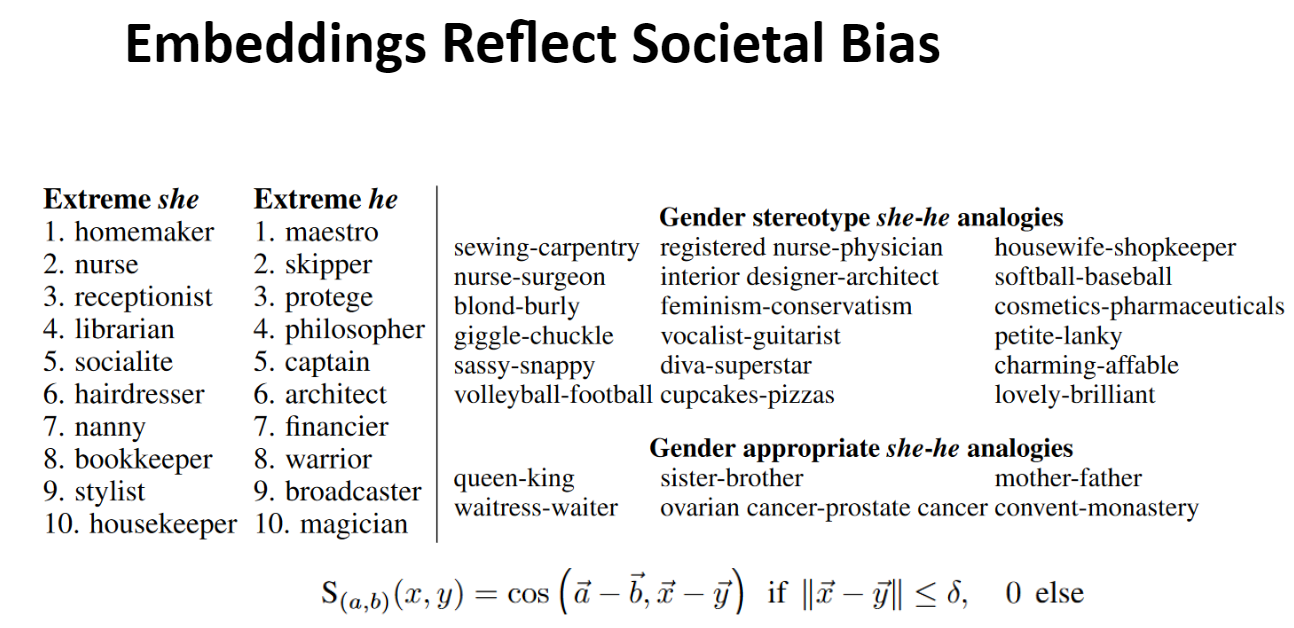
\includegraphics[width=0.8\textwidth]{images/emb_bias.png}
        \end{figure}
        \subsubsection{Identifying and quantifying bias in embeddings}
            \textbf{Aspect of bias is known}: Say "Gender"
            \begin{itemize}
                \item Direct bias - his refers to the alignment of a word vector with the "gender" dimension explicitly extracted from gender-specific word pairs. If a gender-neutral word like "doctor" leans closer to "he" than "she" in the embedding space, it exhibits direct gender bias.
                \newpage
                \begin{mdframed}
                    \begin{itemize}
                        \item We create a matrix with each row representing a word vector from the gendered pairs.
                        \item We apply PCA to identify the most significant components capturing gender.
                        \item We use the first principal component (or a combination of the first few) as the "gender" direction vector $g$.
                        \item We calculate the cosine similarity between \texttt{w\_vec} and $g$:
                        \[ \texttt{direct\_bias(w\_vec)} = \left| \cos(\texttt{w\_vec}, g) \right| \]
                        \item Compute the gender component in elements from $N$ gender neutral words:
                        \[ \texttt{DirectBias} = \frac{1}{|N|} \sum_{w \in N} \left| \cos(w, g) \right| \]
                    \end{itemize}
                \end{mdframed}

                \item Indirect Bias and Perpendicular Component: Indirect bias arises from subtle associations in the training data. These associations might not directly align with the "gender" direction, but they can still influence the position of a word vector in the embedding space.
                \begin{mdframed}
                    \begin{itemize}
                        \item Need to find the component to the perpendicular of the "gender" dimension
                        \item Component of vector $a$ along vector $b$:
                        \begin{itemize}
                            \item Scalar Component: $\texttt{comp}_b(a) = \frac{a \cdot b}{|b|}$
                            \item Vector component: $\texttt{comp}_b(a) \cdot b$
                        \end{itemize}
                        \item $w_g = (w \cdot g)g$, $w_{\perp} = w - w_g$
                        \item IndirectBias $B(w,v) = \frac{w \cdot v - \frac{w_{\perp} \cdot v_{\perp}}{|w_{\perp}| \cdot |v_{\perp}|}}{w \cdot v}$
                    \end{itemize}
                \end{mdframed}
                Modified objective of GloVe to minimize the bias
                \[J = \sum_{i,j=1}^{V} f(X_{ij}) (w_i^T \tilde{w}_j + b_i + \tilde{b}_j - \log X_{ij})^2  + \lambda\cos(w_i, g) + \gamma\cos(\tilde{w}_j, g),\]
            \end{itemize}

    \subsection{FastText}  
        Represent words by sum of of its character n-grams
        \subsubsection{Formulation}
            As in skip-gram, model probability of a context word given a word
            Given word $w$ and context word $w_c$, 
            \[
                P(w_c|w) = P(u_c|v) = \frac{\exp(u_c^T v)}{\sum_{j=1}^{|V|} \exp(u_j^T v)}
            \]
            Given a word $w$, let us denote by $G_w \subset \{1, . . . , G\}$ the set of n-grams appearing in $w$ and itself. We associate a vector representation $z_g$ to each n-gram $g$.
            In FastText the key is to compute feature of a word using its n-grams.\
            \[
                v = \sum_{g \in G} z_g
            \]

            The objective function is the same as in Skip-gram.
    \subsection{Summary - GloVe, Word2Vec, FastText}
        \begin{itemize}
        \item \textbf{Word2vec:}
        \begin{itemize}
            \item \textit{Method:} skip-gram - predicts surrounding words
             and CBOW - predicts center word based on surrounding words.
            \item \textit{Advantages:} Simple and efficient, good at capturing semantic relationships between words.
            \item \textit{Disadvantages:} Doesn't handle rare words well, can be computationally expensive for large datasets.
        \end{itemize}
        \item \textbf{GloVe:}
        \begin{itemize}
            \item \textit{Method:} Analyzes word co-occurrence statistics from a corpus to build word embeddings.
            \item \textit{Advantages:} Often performs well on analogy tasks, considers global word co-occurrence information.
            \item \textit{Disadvantages:} May not capture fine-grained semantic relationships as effectively as word2vec, can be slower to train compared to word2vec.
        \end{itemize}
        \item \textbf{FastText:}
        \begin{itemize}
            \item \textit{Method:} Combines word n-grams (subword information) with word embeddings, allowing it to handle rare words and morphologically related words.
            \item \textit{Advantages:} Handles out-of-vocabulary (OOV) words better than word2vec and GloVe, effective for languages with rich morphology.
            \item \textit{Disadvantages:} Can be more complex to train compared to word2vec, might require more data for optimal performance.
        \end{itemize}
    \end{itemize}
    
    \begin{tabular}{l|cccc}
        \textbf{Feature} & \textbf{Word2vec} & \textbf{GloVe} & \textbf{FastText} \\ \hline
        Captures Semantics & \checkmark & \checkmark & \checkmark \\
        Analogy Tasks  & \checkmark (skip-gram) & \checkmark  & \checkmark \\
        Handles OOV Words & $\times$ & $\times$  & \checkmark \\
        Morphology  & $\times$ & $\times$ & \checkmark  \\
        Efficiency  & \checkmark  & $\times$ & \checkmark \\
        Training Speed  & \checkmark & $\times$  & $\times$ \\
        Context Sensitivity & $\times$  & $\times$ & $\times$ \\
        Syntax Awareness & $\times$ & $\times$ & $\times$ \\
        Fairness  & $\times$ & $\times$ & $\times$ \\
        Reasoning  & $\times$ & $\times$ & $\times$
    \end{tabular}
\section{Language Modelling and Smoothing}
    \begin{itemize}
        \item \textbf{Language modelling is assigning probability to a text-segment/sentence}
        \item \textbf{Usage:}
        \begin{itemize}
            \item \textit{Spell correction:} P(Have you seen this before) vs P(Have you scene this before)
            \item \textit{Speech Recognition:} P(The waiter came running) vs P(The water came running)
            \item \textit{Evaluating generated text:} P(tallest person on earth) vs P(longest person on earth)
            \item \textit{Matching query to documents:} Conditional query-likelihood model. To be discussed later. Which document is a match according to the query’s language model.
        \end{itemize}
    \end{itemize}

    \begin{itemize}
        \item \textbf{Sentence \& Probabilities:}
        \begin{itemize}
            \item We represent a sentence $W$ as a sequence of words: $w_1, w_2, w_3, ..., w_n$.
            \item Language modelLing deals with the probabilities of two key aspects of this sequence:
            \begin{itemize}
                \item $P(W)$: The probability of observing the entire sentence $W$. In other words, how likely is it that this specific sequence of words would appear in natural language?
                \item $P(w_n | w_1, w_2, ..., w_{n-1})$: The probability of encountering the word $w_n$ at the end of the sentence, given the sequence of preceding words $w_1, w_2, ..., w_{n-1}$. This essentially predicts the next word based on the context of previous words.
            \end{itemize}
        \end{itemize}
        \item \textbf{Connection Between $P(W)$ and $P(w_n | w_1, w_2, ..., w_{n-1})$:}
        \begin{itemize}
            \item These two probabilities are fundamentally connected through the chain rule. The chain rule allows us to break down the probability of a complex event (the entire sentence) into the product of probabilities of simpler events (individual words given the preceding context).
        \end{itemize}
        \item \textbf{Chain Rule Example:}
        \begin{itemize}
            \item The chain rule states that the probability of the entire sentence $P(w_1, w_2, w_3, ..., w_n)$ can be expressed as:
            \item $P(w_1, w_2, w_3, ..., w_n) = P(w_1) * P(w_2 | w_1) * P(w_3 | w_1, w_2) * ... * P(w_n | w_1, w_2, ..., w_{n-1})$
            \item Imagine the sentence "go to school". Using the chain rule, we can break down its probability as:
            \item $P(\text{"go to school"}) = P(\text{"go"}) * P(\text{"to"} | \text{"go"}) * P(\text{"school"} | \text{"go", "to"})$
        \end{itemize}
    \end{itemize}

    \subsection{N-gram models}
        \begin{itemize}
            \item \textbf{One way to estimate the probabilities in language modeling is through count-based methods.} This approach leverages the idea that the probability of a word sequence can be determined by how often it appears in a large corpus of text data.
            \item \textbf{Here's a familiar example:}
            \begin{itemize}
                \item $P(w_2 | w_1) = \frac{\text{Count}(w_1w_2)}{\text{Count}(w_1)}$
                \item This equation calculates the probability of encountering word $w_2$ following word $w_1$. We estimate this probability by:
                \begin{itemize}
                    \item Counting the number of times the sequence $w_1w_2$ (bigram) appears in the text data (numerator).
                    \item Dividing this count by the total number of occurrences of word $w_1$ (denominator).
                \end{itemize}
            \end{itemize}
            \item \textbf{Issues with Count-Based Estimates:}
            \begin{itemize}
                \item While intuitive, count-based estimates have limitations:
                \begin{itemize}
                    \item \textit{Data Sparsity:} Language is rich with diverse vocabulary and sentence structures. The training data might not contain every possible word sequence. This can lead to zero probabilities for unseen sequences, making the model unrealistic.
                    \item \textit{Limited Context:} Simple n-gram models (like bigrams and trigrams) only consider a fixed window of preceding words for prediction. They fail to capture long-range dependencies in language, where words far apart in a sentence can influence each other.
                    \item \textit{Ambiguity:} Even with large datasets, some words might have multiple common following words. Count-based methods struggle to capture the nuances of these situations.
                \end{itemize}
            \end{itemize}
        \end{itemize}
    \subsection{Smoothing techniques for LMs}
        We saw how count-based estimates for language models suffer from data sparsity, leading to zero probabilities for unseen n-grams. This is a major problem because natural language is full of variations, and a model shouldn't assign zero probability to something it simply hasn't encountered yet.

        To address this, we use techniques called smoothing. Smoothing essentially adjusts the probabilities estimated from counts to make them more realistic and handle unseen sequences.

        \subsubsection{Add-One Smoothing}
            This is a simple smoothing technique that addresses the zero probability issue. It adds 1 to the numerator (count of the sequence) and the vocabulary size ($|V|$) to the denominator for all n-grams. The smoothed estimate becomes:
            \begin{equation}
                P_{\text{Add-1}}(w_i | w_{i-1}) = \frac{C(w_{i-1} w_i) + 1}{C(w_{i-1}) + |V|}
            \end{equation}
            This ensures that no n-gram gets a zero probability, even if unseen in the training data. However, it has limitations:
            \begin{itemize}
                \item \textbf{Overly Uniform Distribution:} Add-one smoothing distributes the probability mass (total probability of 1) too uniformly across all n-grams, even the rare ones. This can underestimate the probabilities of frequent sequences.
                \item \textbf{Choice of k = 1:} While adding 1 helps, the value of 1 might not be optimal for all scenarios.
            \end{itemize}

        \subsubsection{Add-k Smoothing}
            This is a more general version of add-one smoothing. It replaces adding 1 with adding a value $k$:
            \begin{equation}
            P_{\text{Add-k}}(w_i | w_{i-1}) = \frac{C(w_{i-1} w_i) + k}{C(w_{i-1}) + k |V|}
            \end{equation}
            Here, $k$ is a smoothing parameter that you can tune. It controls the amount of probability mass to be redistributed from frequent n-grams to unseen ones.
            
            \textbf{Choosing the k value}
            Unfortunately, there's no single "best" value for $k$. It depends on the specific dataset and task. Here are some approaches to choose $k$:
            \begin{itemize}
                \item \textbf{Held-out Validation:} Split your data into training and validation sets. Train the model with different $k$ values on the training set and evaluate their performance on the validation set. Choose the $k$ that yields the best performance metric (e.g., perplexity).
                \item \textbf{Linguistic Knowledge:} Some studies suggest setting $k$ based on the vocabulary size or the average number of unseen n-grams encountered during training. However, these methods require domain-specific knowledge.
            \end{itemize}

        \subsubsection{Backoff}
            Tackles the issue of unseen n-grams by gracefully "backing off" to shorter n-grams when the desired n-gram probability estimate isn't reliable. Here's the idea:
            \begin{itemize}
                \item If the specific n-gram (e.g., trigram) you're trying to estimate the probability for is unseen in the training data (count = 0), backoff occurs.
                \item The model then estimates the probability using an $(n-1)$-gram model (bigram in this case). It considers the probability of the last two words $(w_{n-1}, w_n)$ conditioned only on the previous word $(w_{n-2})$.
                \item If the $(n-1)$-gram is also unseen, the model backs off further to an even shorter n-gram model (unigram), and so on.
                \item This process continues recursively until a reliable probability estimate can be obtained from a lower-order n-gram.
            \end{itemize}
        
        \subsubsection{Interpolation}
            Combines probabilities from different n-gram models to create a smoother probability distribution. Here's the approach:
            \begin{itemize}
                \item Instead of relying solely on an n-gram model (e.g., trigram), interpolation considers probabilities from multiple n-gram models (unigram, bigram, and trigram in this case).
                \item Context-based interpolation weights ($\lambda$s) are used to determine the contribution of each n-gram model to the final probability estimate. These weights ($\lambda$s) are typically functions of the previous words in the sequence ($w_{n-2}, w_{n-1}$).
                \item The final probability estimate for a specific n-gram becomes a weighted average of the probabilities from different n-gram models, with weights determined by the context.
            \end{itemize}
            Interpolation allows the model to leverage information from both short and long-range word dependencies, potentially improving prediction accuracy compared to relying solely on a single n-gram model.
        
        \subsubsection{Absolute Discounting}
            Absolute discounting is a technique used to address data sparsity in n-gram language models. It works by subtracting a fixed discount (d) from the counts of n-grams (like bigrams) observed in the training data.
            
            \textbf{Church and Gale experiment on newswire corpus}
            \begin{itemize}
                \item Corpus segmented into two parts (seen/training and held-out) - each with 22M words
                \item From the seen corpus, group together bigrams with different frequencies
                \item For each group, count the average number of occurrences of those bigrams in the held-out corpus
            \end{itemize}
            \begin{figure}[h]
                \centering
                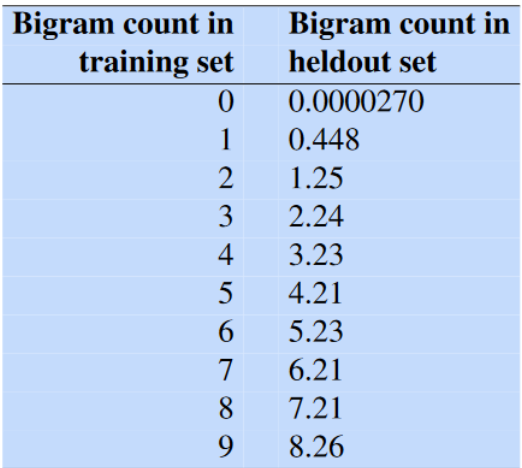
\includegraphics[width=0.8\textwidth]{images/abs_disc.png}
            \end{figure}
            
            
            We can observe that except for the held-out counts for 0 and 1 subtracting 0.75 from bigram counts in the training data provided good estimates for held-out data (unseen bigrams).
            
            Absolute Discounting formalizes the observation by subtracting a fixed discount (0< d < 1) from all bigram counts.
            High-frequency bigrams (reliable counts) are minimally affected by a small discount. Low-frequency bigrams (unreliable counts) benefit from the discount, as it redistributes probability mass to unseen n-grams.

            The formula incorporates the discounted bigram count, unigram probability with interpolation weight, and reflects the trade-off between discounted bigram and unigram probabilities.
            \begin{equation}
                P_{\text{AbsoluteDiscounting}}(w_i | w_{i-1}) = \frac{C(w_{i-1}w_i) - d}{\sum_v C(w_{i-1} v)} + \lambda(w_{i-1})P(w_i)
            \end{equation}

            While a fixed value of 0.75 might work well for some datasets, there are more principled methods to determine the discount value $d$. For instance, Ney et al.'s approach suggests determining $d$ based on unigram counts ($n_1$ and $n_2$).
        
        \subsubsection{Kneser-Ney discounting}
            Similar to Absolute discounting the only difference is how the unigram probability is estimated
            
            The unigram Probability $P(w)$ answers "how likely is $w$ ?"

            Say "Hong Kong" is a very frequent word pair so is "Kong", and "glasses" is less frequent compared to "Hong Kong".
            A standard unigram model would assign higher probability to "Kong" than "glasses", we want to capture the notion that
             "Kong" is frequent in phrase "Hong Kong", but "glasses" has a much wider distribution.
             
           Kneser-Ney method does this by introducing $P_{\text{CONTINUATION}}$  which
           answers the question “How likely is w to appear as a novel continuation?”

           This given by number of word types seen to precede $w$ normalized by the number of words preceding all words
           
            \begin{equation}
                P_{\text{CONTINUATION}}(w) \propto |\{v : C(vw) > 0\}|
            \end{equation}

            \begin{equation}
                P_{\text{CONTINUATION}}(w) = \frac{|\{v : C(vw) > 0\}|}{\sum_{w_0} |\{v : C(vw_0) > 0\}|}
            \end{equation}
            
            The final equation for interpolated Kneser-Ney smoothing for bigrams is:
            \begin{equation}
                P_{\text{KN}}(w_i | w_{i-1}) = \frac{\max(C(w_{i-1}w_i) - d, 0)}{C(w_{i-1})} + \lambda(w_{i-1})P_{\text{CONTINUATION}}(w_i)
            \end{equation}
        
        \subsubsection{Good-Turing Smoothing}
            The idea is to reallocate the probability mass of n-grams that occur $r+ 1$ times in the training data to the n-grams that occur $r$ times.
            
            In particular, reallocate the probability mass of n-grams that were seen once to the n-grams that were never seem before.
            
            Consider the probability mass of all the words that appear $r$ times with new probability model, $N$ denotes the total number of n-grams in the training data.
            ,$r^*$ denotes the adjusted count for n-grams that occur $r$ times, $n_r$, $n_{r+1}$ denotes the number of n-grams that occur $r$, $r+1$ times respectively.
            \begin{align*}
                \sum_{w : C(w) = r} P_{GT}(w) &= \sum_{w^{'} : C(w^{'}) = r+1} P_{MLE}(w^{'}) \\
                \implies r^* \frac{n_{r}}{N} &= (r+1) \frac{n_{r+1}}{N} \\
                \implies r^*  &= \frac{(r + 1) n_{r+1}}{n_r}
            \end{align*}
            \begin{itemize}
                \item As the frequency count ($r$) increases, there are many gaps (0 words with frequency $r$). This makes the Good-Turing (GT) estimate less reliable.
                \item To address this issue, we calculate an adjusted count $Z_r$ from $n_r$ (the number of n-grams seen exactly $r$ times) using the formula $Z_r = \frac{2N_r}{t-q}$.
                \item We then use the log($Z_r$)-vs-$r$ curve to estimate intermediate values for $n_r$.
                \item This is based on the observation that $\log(n_r) = a + b*\log(r)$, where $a$ and $b$ are constants.
                \item For large $r$ values, where the GT estimate is less reliable, we use the fitted value from the log-log plot (also known as the smoothed Good-Turing, or SGT, estimate).
                \item For small $r$ values, where the GT estimate is reliable, we use the GT value.
            \end{itemize}
            \begin{figure}[h]
                \centering
                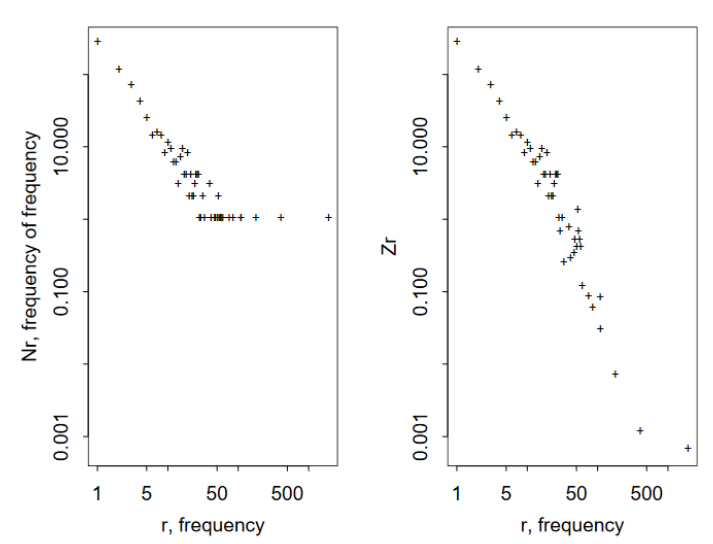
\includegraphics[width=0.8\textwidth]{images/GT.png}
            \end{figure}
            
            Ref: \href{https://nlp.stanford.edu/~wcmac/papers/20050421-smoothing-tutorial.pdf}{https://nlp.stanford.edu/~wcmac/papers/20050421-smoothing-tutorial.pdf}


\section{Discourse in NLP} 
    \begin{itemize}
        \item Coherence
        \begin{itemize}
            \item Ex1 : John took a train from Paris to Istanbul. He likes spinach.
            \item Ex2 : Jane took a train from Paris to Istanbul. She had to attend a conference.
            
            From the above examples we can see there is a structured relation between sentences in Ex2
            compared to Ex1. This structured relation is called Coherence.

            Focuses on salient entities - does not change focus back and forth between multiple entities.
        \end{itemize}
        \textbf{Discourse} is a collection on sentences or text, which has Coherence.
        \item Named Entity Recognition or parsing etc. are inside sentence but coherence is across sentences.
        \item So, Coherence is a higher level of understanding in NLP.
        \item \textbf{Intrinsic features in Discourse}
            \begin{itemize}
                \item Position, order, adjacency and context
                \item 
            \end{itemize}

        \item Coherence as the main characteristic of discourse, for humans we recognize discourse as "it makes sense" or "its relevant".
        \item This is used in Essay grading, summarization, detecting mental health.
        \item A coherent discourse must have meaningful connections(i.e. coherence relations).
        \item Discourse Relations and Connectives - may or may not be explicitly seen.
        \item Some discourse connectives are Synchronous, Reason, Contrast, Conjunction.
        \item How check the extent of Coherence.
        \begin{itemize}
            \item Lexical Chains: Often discussed as cohesion indicator, implemented systems, but not used in text quality tasks.
            Find all words that refer to the same topic and find the correct sense of the words.
            \item Centring theory
            \item Entity Grid: A table with entities in rows and columns, with cells indicating the presence of a relation between entities.
            \item Local coherence detection : Embedding based method: Coherence of thee text is the average similarity over consecutive sentence pair after representing a sentence
             using the LSAS vectors of its words.
            \item Local coherence discriminator - contrastive loss
            
        \end{itemize}
    \end{itemize}
\end{document}
